\chapter{Implementacija i korisničko sučelje}
		
		
		\section{Korištene tehnologije i alati}
		
			 
			 Za potrebe rada na projektu, tim je komunicirao preko aplikacija WhatsApp\footnote{https://www.whatsapp.com/} i Discord\footnote{https://discord.com/}. 
			 Za izradu UML dijagrama, korišten je alat Astah\footnote{https://astah.net/}.
			 Za upravljanje različitim verzijama datoteka korišten je sustav Git\footnote{https://git-scm.com/}.
			 Udaljeni repozitorij projekta nalazi se na platformi Github\footnote{https://github.com/}. Za izradu i testiranje baze korišten je sustav za upravljanje bazama podataka PostgreSQL\footnote{https://www.postgresql.org/}.
			 
			 Kao integrirano razvojno okruženje (IDE) korišten je Intellij IDEA\footnote{https://www.jetbrains.com/idea/}. Ovaj IDE razvio je JetBrains. Koristi se prvenstveno za razvoj softvera napisanog u Javi, Kotlinu i drugim JVM (Java Virtual Machine) jezicima. Preko pluginova nudi podršku i za mnoge druge programske jezike kao što su Python, R, Julia itd. Za potrebe rada na projektu, tim je koristio studentske licence za navedeni IDE preko kojih je moguće koristiti podršku Intellij-a za razne radne okvire (npr. Spring, React).
			 
			 Aplikacija \textit{Ozdravi} napisana je koristeći radni okvir React\footnote{https://react.dev/} za \textit{frontend} te radni okvir Spring\footnote{https://spring.io} za \textit{backend}.
			 \textit{React} je Javascript biblioteka otvorenog koda za izradu korisničkih sučelja. Održavaju ju Meta i zajednica programera i tvrtki. Ova biblioteka brza je i jednostavna za koristiti te se pomoću nje najčešće razvijaju single-page aplikacije. Velika prednost toga je što React omogućuje da se prilikom korištenja sučelja ponovno naslikaju (renderaju) samo dijelovi koji su se izmijenili. Sučelje izrađeno pomoću Reacta sastavljeno je od komponenti koje se mogu ponovno iskoristiti.
			 \textit{Spring} je besplatan radni okvir za razvoj aplikacija u Javi (i drugim jezicima). Vrlo je popularan zbog različitih modula koje nudi čime se znatno ubrzava stvaranje aplikacije. U sklopu izrade ove aplikacije korišteni su Spring Boot (razvoj aplikacije s minimalnom količinom konfiguracija), Spring Security (jednostavna konfiguracija zaštite aplikacije), Spring Data JPA (za lakšu komunikaciju s bazom podataka) i drugi. Za brzo početno podešavanje korištena je stranica Spring initializr\footnote{https://start.spring.io/}.
				
			
			\eject 
		
	
		\section{Ispitivanje programskog rješenja}
			
	
			
			\subsection{Ispitivanje komponenti}
			Ispitivanje komponenti provedeno je koristeći radni okvir \textit{JUnit 5}. Testovi se u tom radnom okviru pišu jednostavno kao zasebne metode. Ako testna metoda dođe do svog kraja, to znači da je test prošao, a ako se dogodi iznimka, test je pao. Osim toga, \textit{JUnit 5} daje velik broj \textit{assertion} metoda koje provjeravaju dane uvjete i bacaju iznimku (ruše test) ako isti nisu ispunjeni. Ovdje je navedeno 7 testova, od jednostavnijih prema složenijima. \\
			
			\noindent \textbf{Prvi test} [\textit{testFetchNonexistentOsoba}] provjerava baca li se odgovarajuća iznimka pri pokušaju dohvaćanja nepostojeće osobe po OIB-u iz baze podataka. 
			\begin{figure}[H]
				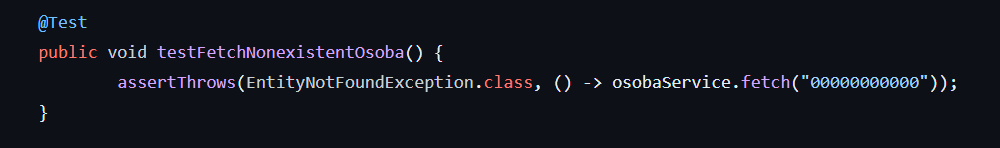
\includegraphics[width=\textwidth]{slike/junit_1.png}
				\caption{Prvi ispitni slučaj}
				\label{fig:junit_1}
			\end{figure}
			% C:\github\Tarantule\dokumentacija\slike
			\noindent \textbf{Drugi test} [\textit{testFetchExistingOsoba}] provjerava dohvaća li se osoba odgovarajućeg imena i prezimena pri dohvaćanju postojeće osobe po OIB-u iz baze podataka.
			\begin{figure}[H]
				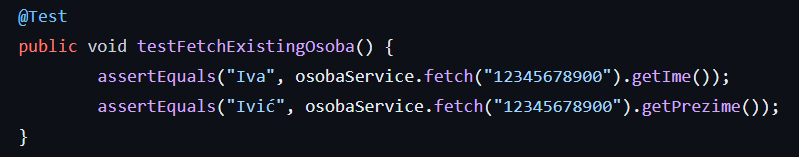
\includegraphics[width=\textwidth]{slike/junit_2.png}
				\caption{Drugi ispitni slučaj}
				\label{fig:junit_2}
			\end{figure}
			
			\noindent \textbf{Treći test} [\textit{testFindOsobaByParentOib}] provjerava funkcionira li metoda za dohvaćanje djece po OIB-u njihovog roditelja na način da usporedi jesu li dobiveni točni OIB-i.
			\begin{figure}[H]
				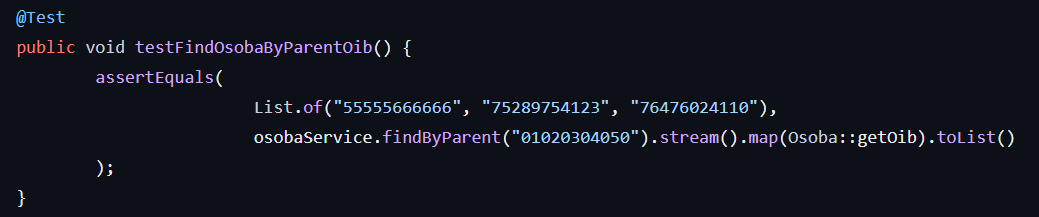
\includegraphics[width=\textwidth]{slike/junit_3.png}
				\caption{Treći ispitni slučaj}
				\label{fig:junit_3}
			\end{figure}
			
			\noindent \textbf{Četvrti test} [\textit{testCreatePoruka}] provjerava može li se dodati validna poruka i hoće li funkcija za stvaranje poruke vratiti dodani objekt.
			\begin{figure}[H]
				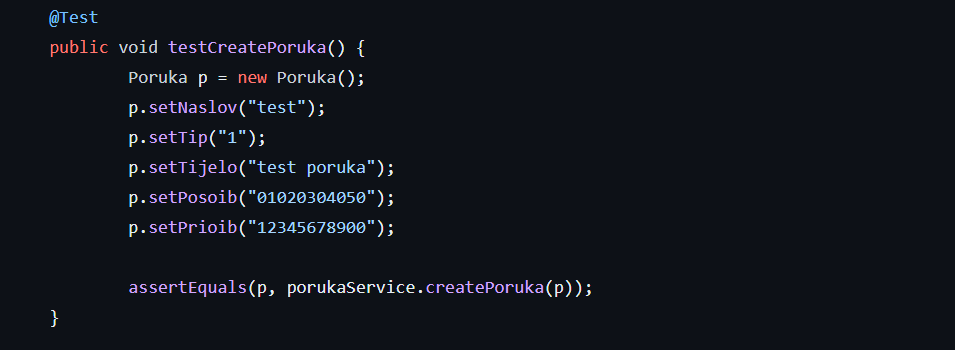
\includegraphics[width=\textwidth]{slike/junit_4.png}
				\caption{Četvrti ispitni slučaj}
				\label{fig:junit_4}
			\end{figure}
			
		 	\noindent \textbf{Peti test} [\textit{testDeletePoruka}] provjerava funkcionira li metoda za brisanje poruke iz baze na način da provjeri vraća li ista objekt s točnim identifikatorom te hoće li nakon toga pokušaj dohvaćanja poruke sa (sada nepostojećim) identifikatorom uzrokovati iznimku jer objekta više nema.
		 	\begin{figure}[H]
		 		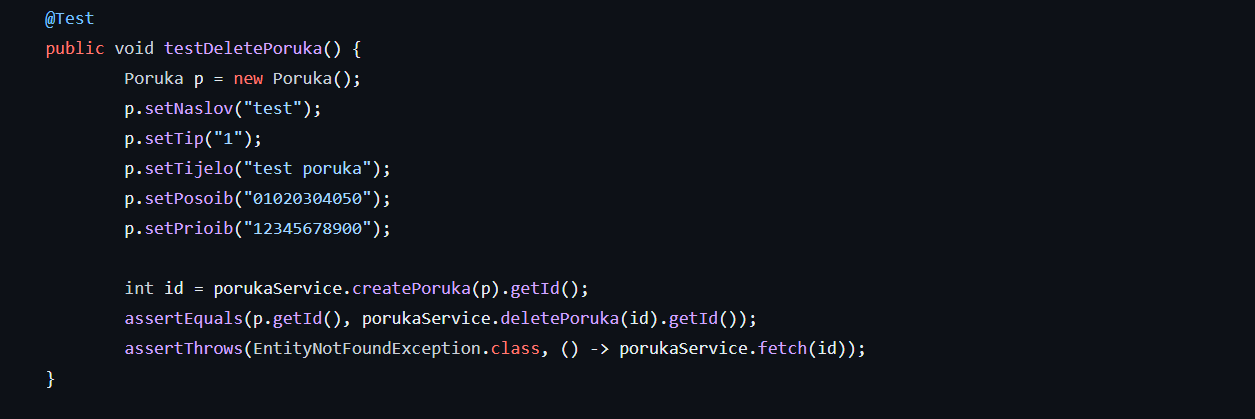
\includegraphics[width=\textwidth]{slike/junit_5.png}
		 		\caption{Peti ispitni slučaj}
		 		\label{fig:junit_5}
		 	\end{figure}
		 	
		 	\noindent \textbf{Šesti test} [\textit{testPorukaBetweenPeople}] provjerava je li moguće ispravno dohvatiti poruke u razgovoru između dvoje ljudi tako da stvori novu poruku između dvoje ljudi i zatim provjeri je li ona među porukama koje vraća testirana metoda. 
		 	\begin{figure}[H]
		 		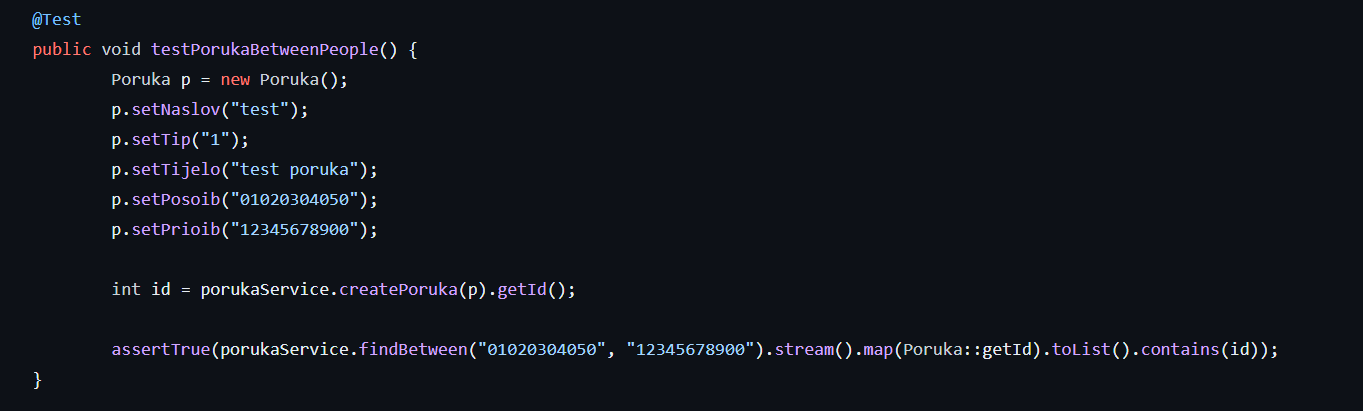
\includegraphics[width=\textwidth]{slike/junit_6.png}
		 		\caption{Šesti ispitni slučaj}
		 		\label{fig:junit_6}
		 	\end{figure}
		 	
		 	\noindent \textbf{Sedmi test} [\textit{testFindUnassignedOsoba}] provjerava metodu koja služi za pronalaženje svih osoba bez doktora/pedijatra. U bazu se doda osoba bez doktora, provjeri se da testirana metoda vraća tu osobu, zatim se osobi doda doktor i konačno se opet poziva testirana metoda i provjeri se da ona ovaj puta ne vraća osobu (jer ona sada ima doktora). 
		 	\begin{figure}[H]
		 		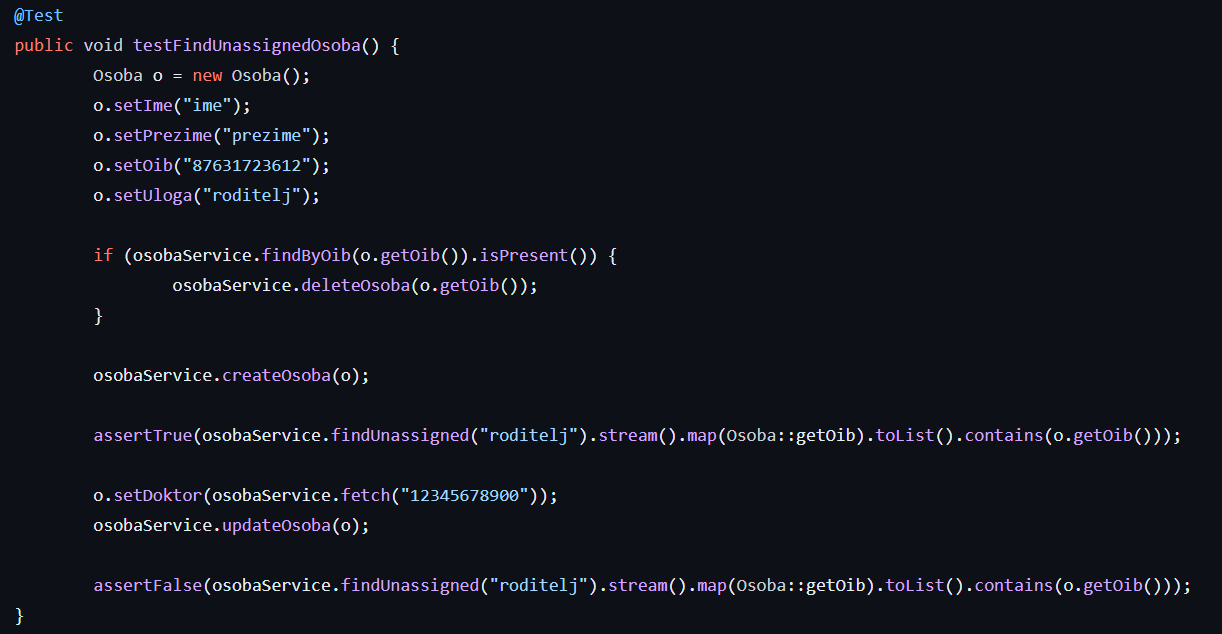
\includegraphics[width=\textwidth]{slike/junit_7.png}
		 		\caption{Sedmi ispitni slučaj}
		 		\label{fig:junit_7}
		 	\end{figure}
			
			\subsection{Ispitivanje sustava}
			
			Testovi su izvršeni pomoću Selenium IDE ekstenzije za Google Chrome. Selenium IDE omogućava automatsko testiranje funkcionalnosti web stranica. Ovaj pristup olakšava identifikaciju grešaka i poboljšava efikasnost procesa testiranja, pružajući preciznost i brzinu u otkrivanju potencijalnih problema.\\ 
				Sam proces testiranja sastoji se od snimanja korisnikovih akcija koje se zatim spremaju kao test. Svaki test moguće je višetruko pokretat te mijenjat unesene parametre. U dokumentaciji je prikazano i opisano testiranje četiri osnovna obrasca uporabe (UC2, UC7, UC24, UC5).\\
			
			\noindent \textbf{Prvi test} provjerava proces prijave u sustav već registriranog korisnika (UC2 - Prijavi se). Tijek testiranja:\\
			Ulazi: 
			\begin{enumerate}
				\item Otvaranje web stranice u pregledniku.
				\item Pritisak na gumb „Prijava“.
				\item Pritisak polja „oib“.
				\item Unos OIB-a postojećeg korisnika.
				\item Pritisak polja „password“
				\item Unos lozinke postojećeg korisnika.
				\item Pritisak na gumb „prijava“.
			\end{enumerate}
			
			\noindent Očekivani rezultat: prikaz stranice korisničkog profila.\\
			Rezultat: očekivani rezultat je zadovoljen i aplikacija prolazi test.
			
			\begin{figure}[H]
				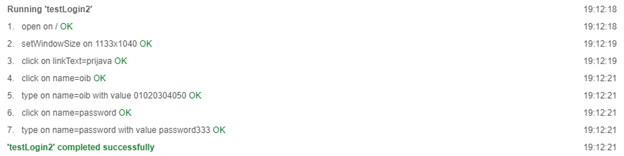
\includegraphics[width=\textwidth]{slike/prijavaUSustav.PNG} %veličina u odnosu na širinu linije
				\caption{Rezultati prvog ispitnog slučaja}
				\label{fig:prijavaTest} %label mora biti drugaciji za svaku sliku
			\end{figure}
			\eject 
		
		\noindent \textbf{Drugi test} provjerava pregled podataka o naručenom specijalističkom pregledu (UC7). \\
			Ulazi: 
		\begin{enumerate}
			\item Odabir profila.
			\item Odabir poruke s naslovom "Naručen pregled".
			\item Pritisak kursorom na kartu, pomicanje kotačića na mišu.
			\item Pritisak kursorom na jednu od označenih bolnica.
		\end{enumerate}
		
		\noindent Očekivani rezultati:\\ Prikazuje se karta sa svim bolnicama iz baze podataka koje su u blizni stanovanja pacijenta. Na karti je moguće mijenjati visinu i poziciju pogleda te otvoriti ikonu s nazivom bolnice.\\
		Rezultati: očekivani rezultat je zadovoljen i aplikacija prolazi test.
		
		\begin{figure}[H]
			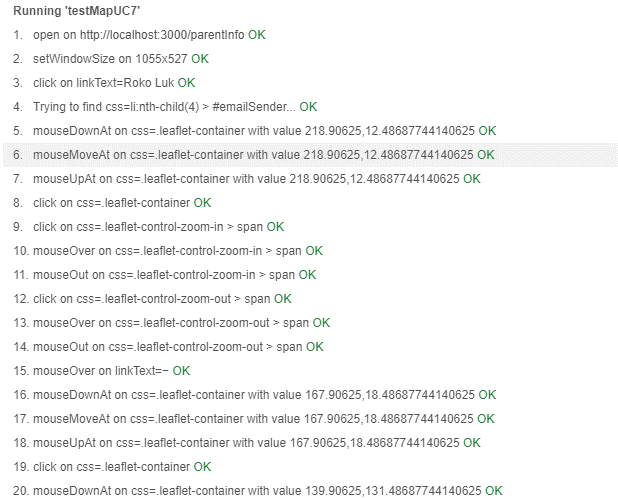
\includegraphics[width=\textwidth]{slike/pregledNaručivanja.PNG} %veličina u odnosu na širinu linije
			\caption{Rezultati drugog ispitnog slučaja}
			\label{fig:pregledKarteTest} %label mora biti drugaciji za svaku sliku
		\end{figure}
		\begin{figure}[H]
			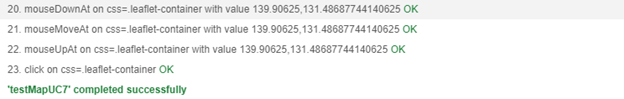
\includegraphics[width=\textwidth]{slike/pregledNaručivanja2.PNG} %veličina u odnosu na širinu linije
			\caption{Rezultati drugog ispitnog slučaja}
			\label{fig:pregledKarteTest2} %label mora biti drugaciji za svaku sliku
		\end{figure}
		
		
		\noindent \textbf{Treći test} provjerava akciju propisivanja bolovanja roditelju (UC24).\\
		Ulazi:
		\begin{enumerate}
			\item Odabir profila roditelja.
			\item Pritisak na „Nova poruka.
			\item Unos teksta poruke.
			\item Označavanje opcije „Bolovanje roditelja“.
			\item Pritisak gumba "Pošalji".
		\end{enumerate}
		Očekivani rezultati:\\Prikaz profila roditelja s novom porukom naziva "dijagnoza". Odabirom te poruke prikazuje se prikaz za čitanje poruke u kojoj vidimo sadržaj i na dnu tekst „Odobreno bolovanje“.\\
		Rezultat: Očekivani rezultat je zadovoljen. Aplikacija je prošla test.
		
		\begin{figure}[H]
			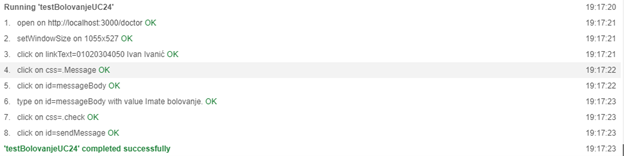
\includegraphics[width=\textwidth]{slike/propisivanjeBolovanja.PNG} %veličina u odnosu na širinu linije
			\caption{Rezultati trećeg ispitnog slučaja}
			\label{fig:propisivanjeBolovanjaTest} %label mora biti drugaciji za svaku sliku
		\end{figure}
		\eject 
		
		\noindent \textbf{Četvrti test} provjerava izmjenu osobnih podataka na stranici roditelja/djeteta (UC 5).\\
		Ulazi:
		\begin{enumerate}
			\item Odabir profila roditelja/djeteta.
			\item Pritisak ikone za izmjenu podataka.
			\item Odabir polja za izmjenu.
			\item Unos novih podataka.
			\item Pritisak na gumb "spremi.
		\end{enumerate}
		Očekivani rezultati:\\ Prikazuje se stranica korisničkog profila. Po otvaranju prozora s osobnim podatcima prikazuju se ažurirani podatci.\\
		Rezultati: Očekivani rezultat je zadovoljen. Aplikacija je prošla test.
		
		\begin{figure}[H]
			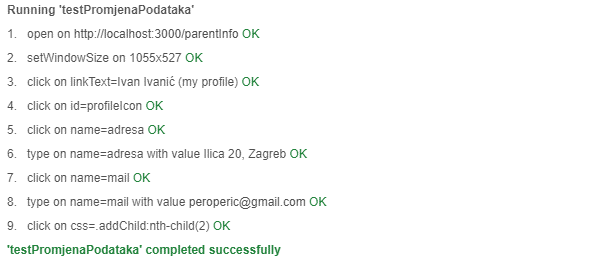
\includegraphics[width=\textwidth]{slike/promjenaPodataka.PNG} %veličina u odnosu na širinu linije
			\caption{Rezultati četvrtog ispitnog slučaja}
			\label{fig:promjenaPodatakaTest} %label mora biti drugaciji za svaku sliku
		\end{figure}
		\eject
		
		Poslijednjim testom prikazujemo kako sustav reagira ukoliko test ne prolazi. Test je proveden ponovnim pokretanjem prvog testa, no ovaj put s neispravnom lozinkom. Očekivani izlaz je neuspješna prijava korisnika te prikaz poruke o pogrešci.
		
		\begin{figure}[H]
			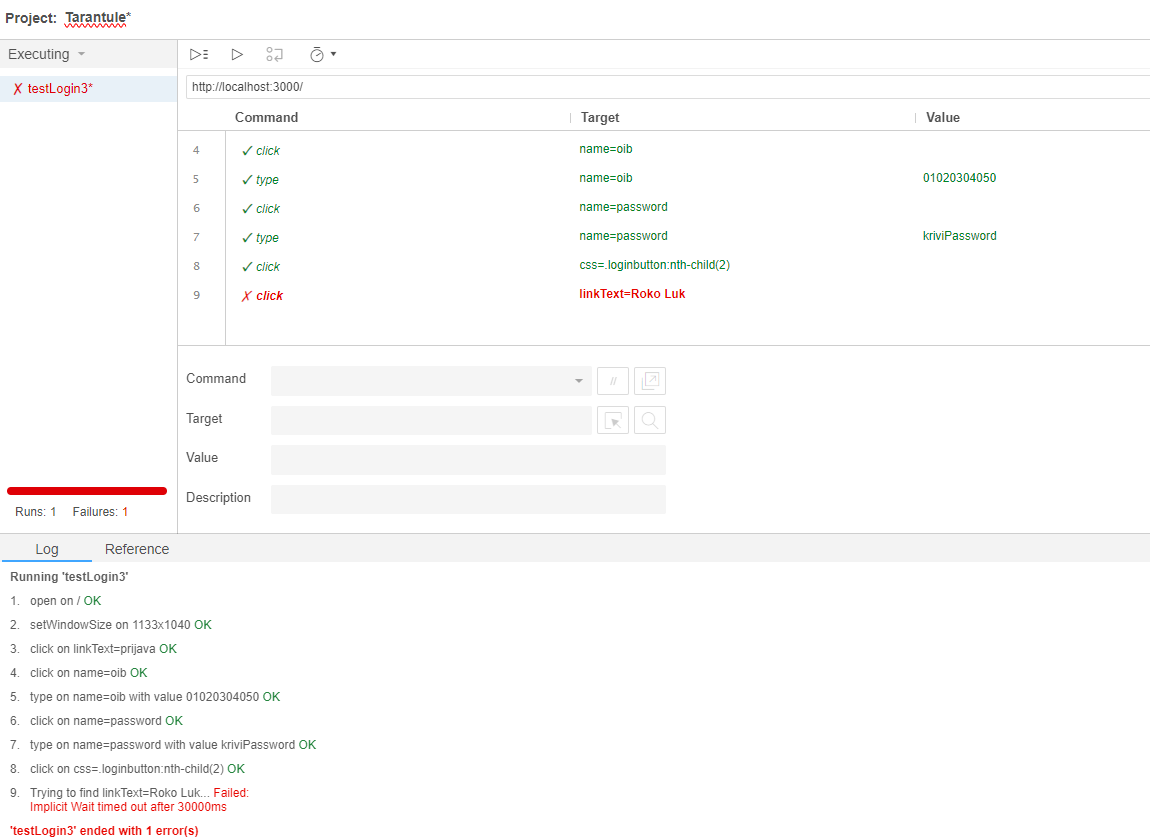
\includegraphics[width=\textwidth]{slike/neispravnaPrijava.PNG} %veličina u odnosu na širinu linije
			\caption{Rezultati i parametri petog ispitnog slučaja}
			\label{fig:neispravnaPrijavaTest} %label mora biti drugaciji za svaku sliku
		\end{figure}
		\eject
		
		\section{Dijagram razmještaja}
			
			 
			 Dijagram razmještaja je strukturni UML dijagram koji opisuje topologiju sustava i prikazuje odnos sklopovskih i programskih dijelova. Na slici \ref{fig:dijagramrazmjestaja} prikazan je specifikacijski dijagram razmještaja aplikacije. Na čvoru koji predstavlja korisnički uređaj nalazi se web preglednik (artefakt) korisnika. On preko HTTPS protoka komunicira s poslužiteljem. Poslužitelj pruža uslugu poslužitelja frontenda, backenda te baze podataka. Sve te usluge mogu međusobno komunicirati slanjem zahtjeva.
			 
			 \begin{figure}[H]
			 	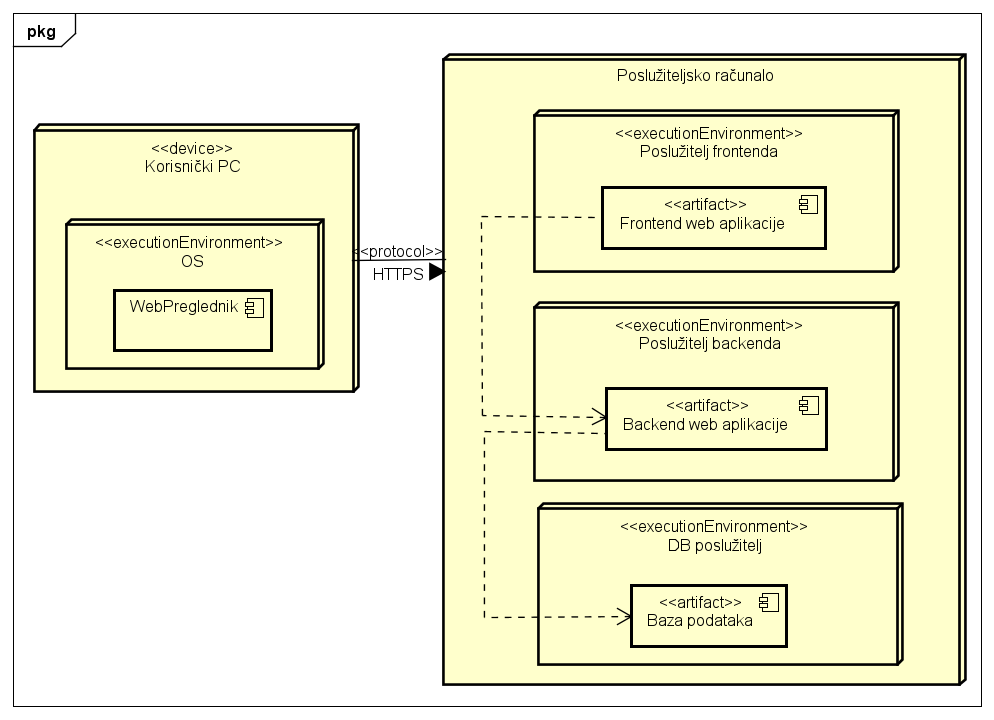
\includegraphics[width=\textwidth]{dijagrami/Dijagram razmjestaja.PNG} %veličina u odnosu na širinu linije
			 	\caption{Dijagram razmještaja}
			 	\label{fig:dijagramrazmjestaja} %label mora biti drugaciji za svaku sliku
			 \end{figure}
			
			\eject 
		
		\section{Upute za puštanje u pogon}
		
			\textbf{\textit{dio 2. revizije}}\\
		
			 \textit{U ovom poglavlju potrebno je dati upute za puštanje u pogon (engl. deployment) ostvarene aplikacije. Na primjer, za web aplikacije, opisati postupak kojim se od izvornog kôda dolazi do potpuno postavljene baze podataka i poslužitelja koji odgovara na upite korisnika. Za mobilnu aplikaciju, postupak kojim se aplikacija izgradi, te postavi na neku od trgovina. Za stolnu (engl. desktop) aplikaciju, postupak kojim se aplikacija instalira na računalo. Ukoliko mobilne i stolne aplikacije komuniciraju s poslužiteljem i/ili bazom podataka, opisati i postupak njihovog postavljanja. Pri izradi uputa preporučuje se \textbf{naglasiti korake instalacije uporabom natuknica} te koristiti što je više moguće \textbf{slike ekrana} (engl. screenshots) kako bi upute bile jasne i jednostavne za slijediti.}
			
			
			 \textit{Dovršenu aplikaciju potrebno je pokrenuti na javno dostupnom poslužitelju. Studentima se preporuča korištenje neke od sljedećih besplatnih usluga: \href{https://aws.amazon.com/}{Amazon AWS}, \href{https://azure.microsoft.com/en-us/}{Microsoft Azure} ili \href{https://www.heroku.com/}{Heroku}. Mobilne aplikacije trebaju biti objavljene na F-Droid, Google Play ili Amazon App trgovini.}
			
			
			\eject 